\documentclass[UTF8,fontset=none]{ctexart}

% Portable CJK font selection for Overleaf / macOS / Windows / Linux.
% The first installed font in this list will be used automatically.
\newcommand{\UseScheduleCJKFont}[1]{%
  \setCJKmainfont{#1}%
  \setCJKfamilyfont{schedulefang}{#1}%
}
\IfFontExistsTF{Noto Serif CJK SC}{
  \UseScheduleCJKFont{Noto Serif CJK SC}
}{
  \IfFontExistsTF{Songti SC}{
    \UseScheduleCJKFont{Songti SC}
  }{
    \IfFontExistsTF{STSong}{
      \UseScheduleCJKFont{STSong}
    }{
      \IfFontExistsTF{SimSun}{
        \UseScheduleCJKFont{SimSun}
      }{
        \IfFontExistsTF{Source Han Serif SC}{
          \UseScheduleCJKFont{Source Han Serif SC}
        }{
          \UseScheduleCJKFont{FandolSong-Regular}
        }
      }
    }
  }
}
\newcommand{\fangsong}{\CJKfamily{schedulefang}}
\usepackage[a4paper,landscape,left=8mm,right=8mm,top=8mm,bottom=8mm]{geometry}
\usepackage[table]{xcolor}
\usepackage{tabularx,array}
\usepackage{needspace}
\usepackage{hyperref}
\usepackage{pdfpages}

\definecolor{scheduleblue}{HTML}{4472C4}
\definecolor{schedulelight}{HTML}{B4C6E7}
\definecolor{schedulepale}{HTML}{DDEBF7}

\pagestyle{empty}
\setlength{\parindent}{0pt}
\setlength{\tabcolsep}{2.2pt}
\setlength{\arrayrulewidth}{0.45pt}
\renewcommand{\arraystretch}{1.28}
\setlength{\extrarowheight}{0.8pt}
\emergencystretch=3em

\newcolumntype{C}[1]{>{\centering\arraybackslash}p{#1}}
\newcolumntype{Y}{>{\centering\arraybackslash}X}
\newcommand{\ScheduleColSpec}{|C{1.65cm}|C{1.75cm}|Y|C{2.20cm}|C{1.70cm}|C{2.20cm}|C{1.80cm}|C{1.70cm}|}

\newcommand{\ScheduleTitle}[1]{%
  \begin{tabularx}{\textwidth}{|C{1.65cm}|C{1.75cm}|Y|C{2.20cm}|C{1.70cm}|C{2.20cm}|C{1.80cm}|C{1.70cm}|}
  \multicolumn{8}{|c|}{\begin{minipage}[c][10mm][c]{0.975\textwidth}\centering\fangsong\bfseries\fontsize{14pt}{16pt}\selectfont #1\end{minipage}}\\\hline
  \end{tabularx}\vspace{1.2mm}
}

\newcommand{\SessionTitle}[1]{%
  \rowcolor{scheduleblue}\multicolumn{8}{|c|}{\begin{minipage}[c][9.5mm][c]{0.975\textwidth}\centering\color{white}\fangsong\bfseries\fontsize{8.7pt}{10.5pt}\selectfont #1\end{minipage}}\\\hline
}
\newcommand{\HeaderRow}{\bfseries 时间 & 报告人 & 题目 & 论文编号 & 辅导老师 & 质疑同学 & 提问老师 & 巡回点评 \\\hline}
\newcommand{\HeaderRowOnsite}{\bfseries 时间 & 报告人 & 题目 & 论文编号 & 辅导老师 & 质疑同学 & 提问老师 & \bfseries 巡回点评\newline（现场） \\\hline}
\newcommand{\ReportBlue}[8]{\rowcolor{schedulelight}#1 & #2 & #3 & #4 & #5 & #6 & #7 & #8 \\\hline}
\newcommand{\ReportWhite}[8]{#1 & #2 & #3 & #4 & #5 & #6 & #7 & #8 \\\hline}
\newcommand{\BreakRow}[2]{\rowcolor{schedulelight}#1 & \multicolumn{7}{c|}{#2} \\\hline}
\newcommand{\BlockGap}{\vspace{2.2mm}}

\newcommand{\DebateHeader}{%
  \rowcolor{schedulepale}\bfseries 场次 & 序号 & 辩论环节 & \multicolumn{4}{c|}{参赛学生（正反方各4人）} & 点评老师 \\\hline
}
\newcommand{\DebateRow}[5]{#1 & #2 & #3 & \multicolumn{4}{c|}{#4} & #5 \\\hline}



\begin{document}

% 第1页
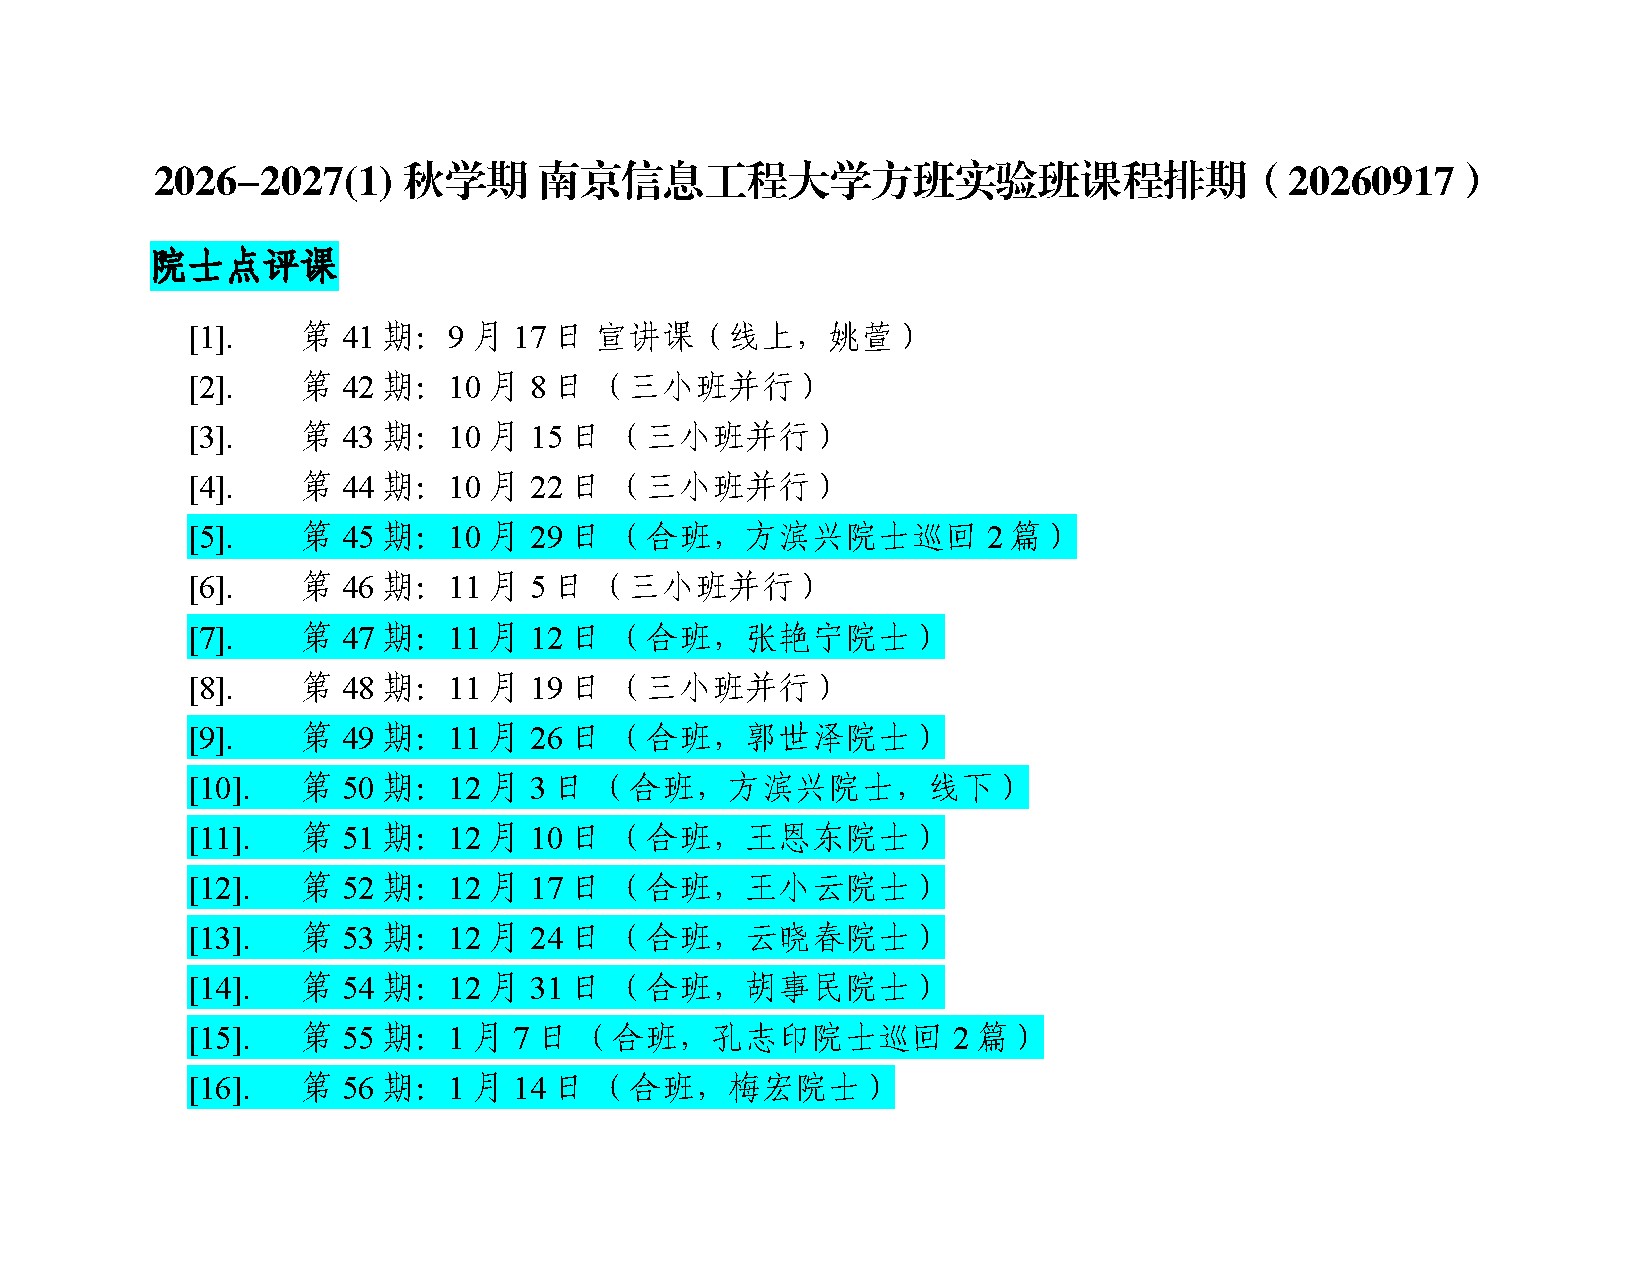
\includepdf[
  pages=1,
  fitpaper=true,
  pagecommand={}
]{课表目录.pdf}

\fangsong\fontsize{7.2pt}{9.2pt}\selectfont

% 第2-4页
% 由原 Excel 课程表转换。通常只需要编辑本文件；版式在 main.tex 中。
% 每个报告用 \ReportBlue 或 \ReportWhite，共 8 个参数：时间、报告人、题目、论文编号、辅导老师、质疑同学、提问老师、巡回点评。

\ScheduleTitle{2026-2027年秋季学期南信大方班实验班课程表}


%%%%%院士课


%方滨兴 10月29日

\Needspace{7.5cm}
\begin{tabularx}{\textwidth}{|C{1.65cm}|C{1.75cm}|Y|C{2.20cm}|C{1.70cm}|C{2.20cm}|C{1.80cm}|C{1.70cm}|}
\SessionTitle{南京信息工程大学实验班第45期课程（10月29日）报告次序表（主点评老师：待定，副点评老师：待定）\newline 腾讯会议号：991-3530-5466 线下课室：临江楼D区报告厅}
\HeaderRow

\ReportBlue{18:00-18:50}{李升冉}
{EM Eye: Characterizing Electromagnetic
Side-channel Eavesdropping on Embedded Cameras\newline EM Eye：嵌入式摄像头中电磁
侧信道窃听的特征分析}
{南信大-45-1-1}
{黄文斌}
{黄嘉乐、丁欣、袁韵涵、薛传朝、钟玉文}
{}{/}

\ReportWhite{18:50-19:40}{丁欣}
{Generative Image Steganography with  Minimum-Distance Guidance\newline 基于最小距离引导的生成式图像隐写}
{南信大-45-1-2}
{张翔}
{鲁懿、赵浩斌、罗靖昇、吴雨健、蒋承睿}
{}{/}

\BreakRow{19:40-19:50}{课间休息}

\ReportWhite{19:50-20:40}{李想}
{SELFDEFEND: LLMs Can Defend Themselves against Jailbreaking in a Practical Manner\newline }
{南信大-45-1-3}
{付章杰}
{董康、李嘉诚、周佳恩、张鑫祺、陆萍萍}
{}{方滨兴}

\ReportBlue{20:40-21:30}{赵宇阳}
{RBLJAN: Robust Byte-Label Joint Attention Network for Network Traffic Classification\newline}
{南信大-45-1-4}
{刘腾骏}
{赵德志、周蕊、朱嘉睿、仉俊杰、张耀腾}
{}{方滨兴}
\end{tabularx}
\BlockGap




%张艳宁 11月12日

\Needspace{7.5cm}
\begin{tabularx}{\textwidth}{|C{1.65cm}|C{1.75cm}|Y|C{2.20cm}|C{1.70cm}|C{2.20cm}|C{1.80cm}|C{1.70cm}|}
\SessionTitle{南京信息工程大学实验班第47期课程（11月12日）报告次序表（主点评老师：张艳宁 院士，副点评老师：待定）\newline 腾讯会议号：991-3530-5466 线下课室：临江楼D区报告厅}
\HeaderRow

\ReportBlue{18:00-18:50}{范泽楠}
{Circumventing shortcuts in audio-visual deepfake detection datasets with unsupervised learning\newline }
{南信大-47-1-1}
{宋甫元}
{周京濮、陆宇竹、孙晨明、张泽浩、谢宸亮}
{}{/}

\ReportWhite{18:50-19:40}{侯睿}
{More Than What Was Chosen: LLM-based Explainable Recommendation Beyond Noisy User Preferences\newline }
{南信大-47-1-2}
{陈先意}
{葛文武、林志鹏、郑宇博、孙孟凡、柳敏烊}
{}{/}

\BreakRow{19:40-19:50}{课间休息}

\ReportWhite{19:50-20:40}{柳敏烊}
{A Multi-Agent Collaboration via Evolving Orchestration\newline 基于演化编排的多智能体协作}
{南信大-47-1-3}
{付章杰}
{刘云飞、耿硕硕、孙祖林、蔡正、胥茗宝}
{}{/}

\ReportBlue{20:40-21:30}{陈佳杰}
{Harnessing Vision-Language Models for Time Series Anomaly Detection\newline}
{南信大-47-1-4}
{陈先意}
{王贵婵、赵泽磊、刘文海、刘孟坤、李孟豪}
{}{/}
\end{tabularx}
\BlockGap


%郭世泽 11月26日

\Needspace{7.5cm}
\begin{tabularx}{\textwidth}{|C{1.65cm}|C{1.75cm}|Y|C{2.20cm}|C{1.70cm}|C{2.20cm}|C{1.80cm}|C{1.70cm}|}
\SessionTitle{南京信息工程大学实验班第49期课程（11月26日）报告次序表（主点评老师：郭世泽 院士，副点评老师：待定）\newline 腾讯会议号：991-3530-5466 线下课室：临江楼D区报告厅}
\HeaderRow

\ReportBlue{18:00-18:50}{赵泽磊}
{SAFE RLHF: SAFE REINFORCEMENT LEARNING FROM HUMAN FEEDBACK\newline }
{南信大-49-1-1}
{姜琴}
{田嘉鑫、吴春雪、尹琨鹏、高豪博、杜佳敏}
{}{/}

\ReportWhite{18:50-19:40}{杨荣发}
{Test-Time Backdoor Detection for Object Detection Models\newline }
{南信大-49-1-2}
{闫雷鸣}
{陈谭浩嵩、王睿轩、张宇慧、高栋森、侯睿}
{}{/}

\BreakRow{19:40-19:50}{课间休息}

\ReportWhite{19:50-20:40}{罗靖昇}
{PoisonedRAG: Knowledge Corruption Attacks to Retrieval-Augmented Generation of Large Language Models\newline }
{南信大-49-1-3}
{崔琦}
{关嘉林、康梦豪、陈佳杰、赵宇阳、李慧敏}
{}{/}

\ReportBlue{20:40-21:30}{裴甲豪}
{A Wolf in Sheep’s Clothing Practical Black-box Adversarial Attacks for Evading Learning-based Windows Malware Detection in the Wild \newline 披着羊皮的狼：真实环境下针对学习型 Windows 恶意软件检测的实用黑盒逃逸攻击}
{南信大-49-1-4}
{付章杰}
{李想、孙一鸣、王少宇、石诗思、杨冬瑞}
{}{/}
\end{tabularx}
\BlockGap



%方滨兴 12月3日


\Needspace{7.5cm}
\begin{tabularx}{\textwidth}{|C{1.65cm}|C{1.75cm}|Y|C{2.20cm}|C{1.70cm}|C{2.20cm}|C{1.80cm}|C{1.70cm}|}
\SessionTitle{南京信息工程大学实验班第50期课程（12月3日）报告次序表（主点评老师：方滨兴 院士，副点评老师：待定）\newline 腾讯会议号：991-3530-5466 线下课室：临江楼D区报告厅}
\HeaderRow

\ReportBlue{18:00-18:50}{周佳恩}
{Contrastive Text-enhanced Transformer for Cross-Domain Sequential Recommendation\newline }
{南信大-50-1-1}
{王一力}
{沈涛涛、张玥宁、吕慎远、魏林东、王钇水}
{}{/}

\ReportWhite{18:50-19:40}{路怀义}
{ChatKBQA A Generate-then-Retrieve Framework for Knowledge Base Question Answering with Fine-tuned Large Language Models\newline }
{南信大-50-1-2}
{李梓强}
{刘铭濠、张继晨、张阳、周旭、徐浩洋}
{}{/}

\BreakRow{19:40-19:50}{课间休息}

\ReportWhite{19:50-20:40}{李孟豪}
{Learning Interpretable Dynamics of Stochastic Complex Systems from Experimental Data\newline }
{南信大-50-1-3}
{王一力}
{朱建华、陈丰羽、吴长凡、路怀义、陈健华}
{}{/}

\ReportBlue{20:40-21:30}{陆晗熙}
{ Catch Me if You Can: Effective Honeypot Placement in Dynamic AD Attack Graphs \newline }
{南信大-50-1-4}
{陈先意}
{范泽楠、杨荣发、杨恺杰、徐渊博、赵咨豪}
{}{/}
\end{tabularx}
\BlockGap



%王恩东：12月10日晚

\Needspace{7.5cm}
\begin{tabularx}{\textwidth}{|C{1.65cm}|C{1.75cm}|Y|C{2.20cm}|C{1.70cm}|C{2.20cm}|C{1.80cm}|C{1.70cm}|}
\SessionTitle{南京信息工程大学实验班第51期课程（12月10日）报告次序表（主点评老师：王恩东 院士，副点评老师：待定）\newline 腾讯会议号：991-3530-5466 线下课室：临江楼D区报告厅}
\HeaderRow

\ReportBlue{18:00-18:50}{徐浩洋}
{SoftCoT: Soft Chain-of-Thought for Efficient Reasoning with LLMs\newline }
{南信大-51-1-1}
{付章杰}
{李梓豪、李义辉、刘雨柯、李京、乔子龙}
{}{/}

\ReportWhite{18:50-19:40}{赵德志}
{CacheBlend: Fast Large Language Model Serving for RAG with Cached Knowledge Fusion\newline }
{南信大-51-1-2}
{李梓强}
{王运动、李升冉、陈文喆、吴世阳、颜子然}
{}{/}

\BreakRow{19:40-19:50}{课间休息}

\ReportWhite{19:50-20:40}{刘文海}
{ExpeL: LLM Agents Are Experiential Learners \newline }
{南信大-51-1-3}
{待定}
{孙焕洛、张鑫、朱毅辰、陆晗熙、黄嘉乐}
{}{/}

\ReportBlue{20:40-21:30}{过杰}
{ FedPE： Adaptive Model Pruning-Expanding forFederated Learning on Mobile Devices\newline }
{南信大-51-1-4}
{陈先意}
{丁欣、袁韵涵、薛传朝、钟玉文、鲁懿}
{}{/}
\end{tabularx}
\BlockGap



%王小云 12月17日
\Needspace{7.5cm}
\begin{tabularx}{\textwidth}{|C{1.65cm}|C{1.75cm}|Y|C{2.20cm}|C{1.70cm}|C{2.20cm}|C{1.80cm}|C{1.70cm}|}
\SessionTitle{南京信息工程大学实验班第52期（12月17日）课程报告次序表（主点评老师：王小云 院士，副点评老师：待定）\newline 腾讯会议号：991-3530-5466 线下课室：临江楼D区报告厅}
\HeaderRow

\ReportBlue{18:00-18:50}{刘雨柯}
{Is PSI Really Faster Than PSU? Achieving Efficient PSU with Invertible Bloom Filters\newline PSI 真的比 PSU 更快吗？——利用可逆布隆过滤器实现高效 PSU}
{南信大-52-1-1}
{姜琴}
{李孟豪、田嘉鑫、吴春雪、尹琨鹏、高豪博}
{}{/}

\ReportWhite{18:50-19:40}{陆宇竹}
{Audio WAtermArk: Dynamic and Harmless Watermark for Black-box Voice Dataset Copyright Protection\newline Audio WAtermArk：面向黑盒语音数据集版权保护的动态无害水印}
{南信大-52-1-2}
{何子文}
{刘铭濠、李梓豪、李义辉、刘雨柯、李京}
{}{/}

\BreakRow{19:40-19:50}{课间休息}

\ReportWhite{19:50-20:40}{郑宇博}
{AutoFHE: Automated Adaption of CNNs for Efficient Evaluation over FHE\newline AutoFHE：自动适配 CNN 以实现 FHE 上的高效评估}
{南信大-52-1-3}
{宋甫元}
{张阳、周旭、李幸、沈涛涛、张继晨}
{}{/}

\ReportBlue{20:40-21:30}{张阳}
{From Interaction to Independence: zkSNARKs for Transparent and Non-Interactive Remote Attestation\newline 从交互到独立：zkSNARKs 实现透明且非交互的远程证明}
{南信大-52-1-4}
{任勇军}
{张玥宁、吕慎远、魏林东、王钇水、杨冬瑞}
{}{/}
\end{tabularx}
\BlockGap



%云晓春：12月24日晚


\Needspace{7.5cm}
\begin{tabularx}{\textwidth}{|C{1.65cm}|C{1.75cm}|Y|C{2.20cm}|C{1.70cm}|C{2.20cm}|C{1.80cm}|C{1.70cm}|}
\SessionTitle{南京信息工程大学实验班第53期课程（12月24日）报告次序表（主点评老师：云晓春 院士，副点评老师：待定）\newline 腾讯会议号：991-3530-5466 线下课室：临江楼D区报告厅}
\HeaderRow

\ReportBlue{18:00-18:50}{周京濮}
{Backdooring Multimodal Learning \newline }
{南信大-53-1-1}
{何子文}
{赵浩斌、罗靖昇、吴雨健、蒋承睿、董康}
{}{/}

\ReportWhite{18:50-19:40}{张宇慧}
{SauronEyes Disentangling Voluminous Logs to Unveil Camouflaged Attack Intentions \newline }
{南信大-53-1-2}
{待定}
{李嘉诚、周佳恩、张鑫祺、陆萍萍、赵德志}
{}{/}

\BreakRow{19:40-19:50}{课间休息}

\ReportWhite{19:50-20:40}{刘铭濠}
{Traffic2Chain: Revealing Covert Multi-Step Attacks Through Unsupervised Traffic Behaviour Correlation \newline }
{南信大-53-1-3}
{待定}
{周蕊、朱嘉睿、仉俊杰、张耀腾、葛文武}
{}{/}

\ReportBlue{20:40-21:30}{袁韵涵}
{Weak-to-Strong Jailbreaking on Large Language Models \newline }
{南信大-53-1-4}
{闫雷鸣}
{林志鹏、郑宇博、孙孟凡、柳敏烊、周京濮}
{}{/}
\end{tabularx}
\BlockGap




%胡事民：12月31日晚


\Needspace{7.5cm}
\begin{tabularx}{\textwidth}{|C{1.65cm}|C{1.75cm}|Y|C{2.20cm}|C{1.70cm}|C{2.20cm}|C{1.80cm}|C{1.70cm}|}
\SessionTitle{南京信息工程大学实验班第54期课程（12月31日）报告次序表（主点评老师：胡事民 院士，副点评老师：待定）\newline 腾讯会议号：991-3530-5466 线下课室：临江楼D区报告厅}
\HeaderRow

\ReportBlue{18:00-18:50}{陈文喆}
{One Prompt Word is Enough to Boost Adversarial Robustness for Pre-trained Vision-Language Models \newline }
{南信大-54-1-1}
{李梓强}
{陆宇竹、孙晨明、张泽浩、谢宸亮、刘云飞}
{}{/}

\ReportWhite{18:50-19:40}{杨恺杰}
{BadThink: Triggered Overthinking Attacks on Chain-of-Thought Reasoning in Large Language Models \newline }
{南信大-54-1-2}
{熊礼治}
{耿硕硕、孙祖林、蔡正、胥茗宝、王贵婵}
{}{/}

\BreakRow{19:40-19:50}{课间休息}

\ReportWhite{19:50-20:40}{李慧敏}
{Distraction is All You Need for Multimodal Large Language Model Jailbreaking\newline }
{南信大-54-1-3}
{李梓强}
{赵泽磊、刘文海、刘孟坤、李孟豪、田嘉鑫}
{}{/}

\ReportBlue{20:40-21:30}{陈丰羽}
{Look Twice Before You Answer: Memory-Space Visual Retracing for Hallucination Mitigation in Multimodal Large Language Models \newline }
{南信大-54-1-4}
{付章杰}
{吴春雪、尹琨鹏、高豪博、杜佳敏、陈谭浩嵩}
{}{/}
\end{tabularx}
\BlockGap



%孔志印：1月7日晚




\Needspace{7.5cm}
\begin{tabularx}{\textwidth}{|C{1.65cm}|C{1.75cm}|Y|C{2.20cm}|C{1.70cm}|C{2.20cm}|C{1.80cm}|C{1.70cm}|}
\SessionTitle{南京信息工程大学实验班第55期课程（1月7日）报告次序表（主点评老师：孔志印 院士，副点评老师：待定）\newline 腾讯会议号：991-3530-5466 线下课室：临江楼D区报告厅}
\HeaderRow

\ReportBlue{18:00-18:50}{尹琨鹏}
{AdvAD: Exploring Non-Parametric Diffusion for Imperceptible Adversarial Attacks \newline }
{南信大-55-1-1}
{陈北京}
{王睿轩、张宇慧、高栋森、侯睿、关嘉林}
{}{孔志印}

\ReportWhite{18:50-19:40}{李幸}
{Red-Teaming LLM Multi-Agent Systems via Communication Attacks \newline }
{南信大-55-1-2}
{付章杰}
{张继晨、张阳、周旭、裴甲豪、沈涛涛}
{}{孔志印}

\BreakRow{19:40-19:50}{课间休息}

\ReportWhite{19:50-20:40}{李义辉}
{Class-feature Watermark: A Resilient Black-box Watermark Against Model Extraction Attacks     \newline  类别特征水印：一种抵御模型提取攻击的鲁棒黑盒水印方法}
{南信大-55-1-3}
{高光勇}
{康梦豪、陈佳杰、赵宇阳、李慧敏、李想}
{}{/}

\ReportBlue{20:40-21:30}{朱毅辰}
{VOID: Defeating Unauthorized Mimicry in Latent Diffusion Models \newline VOID：防御潜在扩散模型中的未经授权身份模仿}
{南信大-55-1-4}
{熊礼治}
{孙一鸣、王少宇、石诗思、杨冬瑞、刘铭濠}
{}{/}
\end{tabularx}
\BlockGap




%梅宏：1月14日晚



\Needspace{7.5cm}
\begin{tabularx}{\textwidth}{|C{1.65cm}|C{1.75cm}|Y|C{2.20cm}|C{1.70cm}|C{2.20cm}|C{1.80cm}|C{1.70cm}|}
\SessionTitle{南京信息工程大学实验班第56期课程（1月14日）报告次序表（主点评老师：梅宏 院士，副点评老师：待定）\newline 腾讯会议号：991-3530-5466 线下课室：临江楼D区报告厅}
\HeaderRow

\ReportBlue{18:00-18:50}{张鑫祺}
{Unlocking the Capabilities of Thought： A Reasoning Boundary Framework to Quantify and Optimize Chain-of-Thought\newline }
{南信大-56-1-1}
{待定}
{张玥宁、吕慎远、魏林东、王钇水、李梓豪}
{}{/}

\ReportWhite{18:50-19:40}{田嘉鑫}
{Chain-of-thought reasoning without prompting \newline 无需提示的思维链推理}
{南信大-56-1-2}
{待定}
{李义辉、刘雨柯、李京、乔子龙、朱建华}
{}{/}

\BreakRow{19:40-19:50}{课间休息}

\ReportWhite{19:50-20:40}{仉俊杰}
{REGENT: A Retrieval-Augmented Generalist Agent That Can Act In-Context in New Environments \newline }
{南信大-56-1-3}
{崔琦}
{陈丰羽、吴长凡、路怀义、陈健华、范泽楠}
{}{/}

\ReportBlue{20:40-21:30}{林志鹏}
{MemAgent: Reshaping Long-Context LLM with Multi-Conv RL-based Memory Agent \newline }
{南信大-56-1-4}
{王晓苏}
{杨荣发、杨恺杰、徐渊博、赵咨豪、王运动}
{}{/}
\end{tabularx}
\BlockGap





% 第5页
\includepdf[
  pages=2,
  fitpaper=true,
  pagecommand={}
]{课表目录.pdf}

% 第6页开始
%%%%%非院士课

%%10月8日 3个班

\Needspace{7.5cm}
\begin{tabularx}{\textwidth}{|C{1.65cm}|C{1.75cm}|Y|C{2.20cm}|C{1.70cm}|C{2.20cm}|C{1.80cm}|C{1.70cm}|}
\SessionTitle{南京信息工程大学实验班第42期课程（10月8日）一班报告次序表（主点评老师：程旭，副点评老师：李梓强）\newline 腾讯会议号：991-3530-5466 线下课室：临江楼A207-208会议室}
\HeaderRow
\ReportBlue{18:00-18:50}{徐渊博}
{GenShield: Unified Detection and Artifact Correction for AI-Generated Images\newline
GenShield：用于人工智能生成图像的统一检测与伪像校正}
{南信大-42-1-1}
{熊礼治}
{乔子龙、朱时修、陈丰羽、吴长凡、路怀义}
{何子文}{/}

\ReportWhite{18:50-19:40}{吕慎远}
{Black-Box Adversarial Attacks on LLM-Based Code Completion\newline 针对基于大语言模型的代码补全的黑盒对抗攻击}
{南信大-42-1-3}
{孟若涵}
{陈健华、范泽楠、杨荣发、杨恺杰、徐渊博}
{何子文}{/}

\BreakRow{19:40-19:50}{课间休息}

\ReportWhite{19:50-20:40}{黄嘉乐}
{Cloak, Honey, Trap: Proactive Defenses Against LLM Agents\newline 隐蔽、诱饵、陷阱：主动防御LLM特工}
{南信大-42-1-2}
{付章杰}
{赵咨豪、王运动、李升冉、陈文喆、吴世阳}
{孟若涵}{/}

\ReportBlue{20:40-21:30}{鲁懿}
{Hiding Images in Diffusion Models by Editing Learned Score Functions \newline 通过编辑学习到的评分函数在扩散模型中隐藏图像}
{南信大-42-1-4}
{张翔}
{颜子然、孙焕洛、张鑫、朱毅辰、陆晗熙}
{孟若涵}{/}
\end{tabularx}
\BlockGap



\Needspace{7.5cm}
\begin{tabularx}{\textwidth}{|C{1.65cm}|C{1.75cm}|Y|C{2.20cm}|C{1.70cm}|C{2.20cm}|C{1.80cm}|C{1.70cm}|}
\SessionTitle{南京信息工程大学实验班第42期课程（10月8日）二班报告次序表（主点评老师：高光勇，副点评老师：崔琦）\newline 腾讯会议号：511-4917-5751 线下课室：临江楼A209-210会议室}
\HeaderRow
\ReportBlue{18:00-18:50}{吴春雪}
{Collaborative Transformers with Multi-LevelForensic Attention for Image ManipulationLocalization\newline
基于多级取证协同注意力Transformer的图像篡改定位}
{南信大-42-2-1}
{檀振山}
{李升冉、陈文喆、吴世阳、颜子然、孙焕洛}
{余佩鹏}{/}

\ReportWhite{18:50-19:40}{蔡正}
{Forensics Adapter: Adapting CLIP for Generalizable Face Forgery Detection \newline Forensics Adapter：用于泛化人脸伪造检测的自适应CLIP}
{南信大-42-2-2}
{张翔}
{张鑫、朱毅辰、陆晗熙、黄嘉乐、丁欣}
{余佩鹏}{/}

\BreakRow{19:40-19:50}{课间休息}

\ReportWhite{19:50-20:40}{谢宸亮}
{When VR Meets BCI: (Un)Observable Brainwave-Aware Privacy Reconstruction in the Metaverse via Unrestricted Inbuilt Motion Sensors\newline 当VR遇见BCI：元宇宙中通过无限制内置运动传感器实现的（不可）可观测脑电波感知隐私重建}
{南信大-42-2-3}
{杨盘隆}
{袁韵涵、薛传朝、钟玉文、鲁懿、赵浩斌}
{周丽贞}{/}

\ReportBlue{20:40-21:30}{颜子然}
{Invisible and Robust Watermarking for AI-generated Image  Provenance  \newline 面向AI生成图像溯源的不可见鲁棒水印方法}
{南信大-42-2-4}
{陈北京}
{罗靖昇、吴雨健、蒋承睿、董康、李嘉诚}
{周丽贞}{/}
\end{tabularx}
\BlockGap


\Needspace{7.5cm}
\begin{tabularx}{\textwidth}{|C{1.65cm}|C{1.75cm}|Y|C{2.20cm}|C{1.70cm}|C{2.20cm}|C{1.80cm}|C{1.70cm}|}
\SessionTitle{南京信息工程大学实验班第42期课程（10月8日）三班报告次序表（主点评老师：熊礼治，副点评老师：袁程胜）\newline 腾讯会议号：634-7226-4550 线下课室：临江楼A213-214会议室}
\HeaderRow
\ReportBlue{18:00-18:50}{关嘉林}
{CodeMark Contextual and Natural Watermarking for Tracing Code Snippet Provenance \newline CodeMark：用于追踪代码片段来源的上下文感知自然水印}
{南信大-42-3-1}
{檀振山}
{周佳恩、张鑫祺、陆萍萍、赵德志、周蕊}
{孟若涵}{/}

\ReportWhite{18:50-19:40}{王钇水}
{Guidance Watermarking for Diffusion Models\newline 面向扩散模型的引导式水印技术 }
{南信大-42-3-2}
{陈北京}
{朱嘉睿、仉俊杰、张耀腾、葛文武、林志鹏}
{孟若涵}{/}

\BreakRow{19:40-19:50}{课间休息}

\ReportWhite{19:50-20:40}{杜佳敏}
{Leafblower: a Leakage Attack Against TEE-Based Encrypted Databases\newline Leafblower：一种针对基于可信执行环境（TEE）的加密数据库的泄露攻击}
{南信大-42-3-3}
{姜琴}
{郑宇博、孙孟凡、柳敏烊、周京濮、陆宇竹}
{沙金锐}{/}

\ReportBlue{20:40-21:30}{石诗思}
{Towards Matchmaking Task Selection with Forward and Backward Secrecy for Medical Crowdsourcing  \newline 面向医疗众包的前向与后向保密任务选择匹配研究}
{南信大-42-3-4}
{宋甫元}
{孙晨明、张泽浩、谢宸亮、刘云飞、耿硕硕}
{沙金锐}{/}
\end{tabularx}
\BlockGap




%%10月15日 3个班


\Needspace{7.5cm}
\begin{tabularx}{\textwidth}{|C{1.65cm}|C{1.75cm}|Y|C{2.20cm}|C{1.70cm}|C{2.20cm}|C{1.80cm}|C{1.70cm}|}
\SessionTitle{南京信息工程大学实验班第43期课程（10月15日）一班报告次序表（主点评老师：尹春勇，副点评老师：付道勇）\newline 腾讯会议号：991-3530-5466 线下课室：临江楼A104-105会议室}
\HeaderRow
\ReportBlue{18:00-18:50}{张继晨}
{Continuous Space-Time Video Resampling with Invertible Motion Steganography\newline 
可逆运动隐藏技术下的连续时空视频重采样}
{南信大-43-1-1}
{张翔}
{孙祖林、蔡正、胥茗宝、王贵婵、赵泽磊}
{檀振山}{/}

\ReportWhite{18:50-19:40}{张玥宁}
{Towards Reliable Verification of Unauthorized Data Usage in Personalized Text-to-Image Diffusion Models \newline 
面向个性化文生图扩散模型的未经授权数据使用可靠验证研究}
{南信大-43-1-2}
{崔萌萌}
{刘文海、刘孟坤、李孟豪、田嘉鑫、吴春雪}
{檀振山}{/}

\BreakRow{19:40-19:50}{课间休息}

\ReportWhite{19:50-20:40}{王贵婵}
{RAP: Resource‑Adaptive Planning for Efficient LLM Tool Calling in Edge Computing \newline 
RAP：面向边缘计算的大语言模型高效工具调用资源自适应规划}
{南信大-43-1-3}
{周丽贞}
{尹琨鹏、高豪博、杜佳敏、陈谭浩嵩、王睿轩}
{刘腾骏}{/}

\ReportBlue{20:40-21:30}{王运动}
{RoPaSS: Robust Watermarking for Partial Screen‑Shooting Scenarios\newline 
面向部分屏幕拍摄场景的鲁棒水印方案}
{南信大-43-1-4}
{王保卫}
{王少宇、石诗思、杨冬瑞、刘铭濠、张继晨}
{刘腾骏}{/}
\end{tabularx}
\BlockGap



\Needspace{7.5cm}
\begin{tabularx}{\textwidth}{|C{1.65cm}|C{1.75cm}|Y|C{2.20cm}|C{1.70cm}|C{2.20cm}|C{1.80cm}|C{1.70cm}|}
\SessionTitle{南京信息工程大学实验班第43期课程（10月15日）二班报告次序表（主点评老师：任勇军，副点评老师：张翔）\newline 腾讯会议号：511-4917-5751 线下课室：	临江楼A106-107会议室}
\HeaderRow
\ReportBlue{18:00-18:50}{高栋森}
{No Way To Steal My Face: Proactive Defense Against Identity-Preserving Personalized Generation \newline 别想偷我的脸：主动防护身份保留的个性化生成}
{南信大-43-2-1}
{袁程胜}
{陈佳杰、赵宇阳、李慧敏、李想、孙一鸣}
{刘腾骏}{/}

\ReportWhite{18:50-19:40}{孙焕洛}
{Oblivious and Privacy-Preserving loT Spatial Range Keyword Query with Dynamic Authorization  \newline 具有动态授权的物联网空间范围关键词查询的遗忘性与隐私保护}
{南信大-43-2-2}
{宋甫元}
{张宇慧、高栋森、魏林东、关嘉林、康梦豪}
{刘腾骏}{/}

\BreakRow{19:40-19:50}{课间休息}

\ReportWhite{19:50-20:40}{魏林东}
{Gaussian Shading: Provable Performance-Lossless Image Watermarking for Diffusion Models
\newline 高斯着色：扩散模型的可证明性能无损图像水印}
{南信大-43-2-3}
{何子文}
{吕慎远、王钇水、侯睿、李梓豪、李义辉}
{乔塨哲}{/}

\ReportBlue{20:40-21:30}{李梓豪}
{IP-Adapter Is All You Need: Towards Fine-Tuning-Free Diffusion-Based Talking Face Generation\newline IP-Adapter: 面向无需微调的扩散式说话人脸生成范式 }
{南信大-43-2-4}
{袁程胜}
{刘雨柯、李京、乔子龙、朱时修、陈丰羽}
{乔塨哲}{/}
\end{tabularx}
\BlockGap


\Needspace{7.5cm}
\begin{tabularx}{\textwidth}{|C{1.65cm}|C{1.75cm}|Y|C{2.20cm}|C{1.70cm}|C{2.20cm}|C{1.80cm}|C{1.70cm}|}
\SessionTitle{南京信息工程大学实验班第43期课程（10月15日）三班报告次序表（主点评老师：陈北京，副点评老师：宋甫元）\newline 腾讯会议号：634-7226-4550 线下课室：临江楼A103会议室}
\HeaderRow
\ReportBlue{18:00-18:50}{刘云飞}
{MarkPlugger: Generalizable Watermark Framework for Latent Diffusion Models without Retraining \newline MarkPlugger: 无需重新训练的可通用化潜在扩散模型水印框架 }
{南信大-43-3-1}
{孟若涵}
{张阳、周旭、李想、沈涛涛、张玥宁}
{乔塨哲}{/}

\ReportWhite{18:50-19:40}{董康}
{WMAdapter: Adding WaterMark Control to Latent Diffusion Models\newline  
水印适配器: 为潜在扩散模型增加水印控制能力}
{南信大-43-3-2}
{熊礼治}
{吴长凡、路怀义、陈健华、范泽楠、杨荣发}
{乔塨哲}{/}

\BreakRow{19:40-19:50}{课间休息}

\ReportWhite{19:50-20:40}{张鑫}
{Diffusion Reconstruction Contrastive Training towards Universal Detection of Diffusion Generated Images\newline 面向扩散生成图像通用检测的扩散重建对比训练}
{南信大-43-3-3}
{何子文}
{杨恺杰、徐渊博、赵咨豪、王运动、李升冉}
{檀振山}{/}

\ReportBlue{20:40-21:30}{赵咨豪}
{Physical Marker: Revealing Invisible Hyperlinks Hidden in Printed Trademarks\newline 
物理标记：揭示印刷商标中隐藏的隐形超链接}
{南信大-43-3-4}
{高光勇}
{陈文喆、吴世阳、颜子然、孙焕洛、张鑫}
{檀振山}{/}
\end{tabularx}
\BlockGap






%%10月22日 3个班

\Needspace{7.5cm}
\begin{tabularx}{\textwidth}{|C{1.65cm}|C{1.75cm}|Y|C{2.20cm}|C{1.70cm}|C{2.20cm}|C{1.80cm}|C{1.70cm}|}
\SessionTitle{南京信息工程大学实验班第44期课程（10月22日）一班报告次序表（主点评老师：待定，副点评老师：韩飞宇）\newline 腾讯会议号：991-3530-5466 线下课室：临江楼A207-208会议室}
\HeaderRow
\ReportBlue{18:00-18:50}{孙一鸣}
{SemBind:Binding Diffusion Watermarks to Semantics Against Black-Box Forgery Attacks\newline SemBind:将扩散水印与语义绑定以对抗黑盒伪造攻击}
{南信大-44-1-1}
{崔琦}
{朱毅辰、陆晗熙、黄嘉乐、丁欣、袁韵涵}
{崔员宁}{/}

\ReportWhite{18:50-19:40}{吴雨健}
{Screen-Shooting Robust Watermark Based on Style Transfer and Structural Re-parameterization    \newline  基于风格迁移与结构重参数化的屏摄鲁棒水印}
{南信大-44-1-2}
{高光勇}
{薛传朝、钟玉文、鲁懿、赵浩斌、罗靖昇}
{崔员宁}{/}

\BreakRow{19:40-19:50}{课间休息}

\ReportWhite{19:50-20:40}{张泽浩}
{DiffLoc: WiFi Hidden Camera Localization Based on Electromagnetic Diffraction     \newline  DiffLoc: WiFi隐藏摄像机的电磁衍射定位}
{南信大-44-1-3}
{黄文斌}
{吴雨健、蒋承睿、董康、李嘉诚、周佳恩}
{何子文}{/}

\ReportBlue{20:40-21:30}{陆萍萍}
{K-Space Bispectrum Steganography for Robust Unlearnable Data \newline K空间双谱隐写: 面向鲁棒不可学习数据的方法}
{南信大-44-1-4}
{孟若涵}
{仉俊杰、张耀腾、葛文武、林志鹏、郑宇博}
{何子文}{/}
\end{tabularx}
\BlockGap



\Needspace{7.5cm}
\begin{tabularx}{\textwidth}{|C{1.65cm}|C{1.75cm}|Y|C{2.20cm}|C{1.70cm}|C{2.20cm}|C{1.80cm}|C{1.70cm}|}
\SessionTitle{南京信息工程大学实验班第44期课程（10月22日）二班报告次序表（主点评老师：待定，副点评老师：王文珍）\newline 腾讯会议号：511-4917-5751 线下课室：	
临江楼A209-210会议室}
\HeaderRow
\ReportBlue{18:00-18:50}{赵浩斌}
{Leaking the Privacy of Groups and More: Understanding Privacy Risks of Cross-App Content  Sharing in Mobile Ecosystem \newline 泄露群组隐私及更多内容: 了解移动的生态系统中跨应用内容共享的隐私风险}
{南信大-44-2-1}
{黄文斌}
{张鑫祺、陆萍萍、赵德志、周蕊、朱嘉睿}
{何子文}{/}


\ReportWhite{18:50-19:40}{朱时修}
{Privacy-Preserving Data Deduplication for Enhancing Federated Learning of Language Models }
{南信大-44-2-3}
{任勇军}
{孙孟凡、柳敏烊、周京濮、陆宇竹、孙晨明}
{何子文}{/}

\BreakRow{19:40-19:50}{课间休息}



\ReportWhite{19:50-20:40}{钟玉文}
{MOVE: Effective and Harmless Ownership Verification via Embedded External Features   \newline MOVE：基于嵌入外部特征的高效无损伤所有权验证}
{南信大-44-2-3}
{付道勇}
{张泽浩、谢宸亮、刘云飞、耿硕硕、孙祖林}
{崔员宁}{/}

\ReportBlue{20:40-21:30}{陈健华}
{FedPoD: Federated Prompt Learning for Weather Foundation Models on Devices \newline  FedPoD：用于设备上的天气基础模型的联合提示学习 }
{南信大-44-2-4}
{田伟}
{蔡正、胥茗宝、王贵婵、赵泽磊、刘文海}
{崔员宁}{/}
\end{tabularx}
\BlockGap


\Needspace{7.5cm}
\begin{tabularx}{\textwidth}{|C{1.65cm}|C{1.75cm}|Y|C{2.20cm}|C{1.70cm}|C{2.20cm}|C{1.80cm}|C{1.70cm}|}
\SessionTitle{南京信息工程大学实验班第44期课程（10月22日）三班报告次序表（主点评老师：待定，副点评老师：姚萱）\newline 腾讯会议号：634-7226-4550 线下课室：临江楼A213-214会议室}
\HeaderRow
\ReportBlue{18:00-18:50}{沈涛涛}
{PRSA: Prompt Stealing Attacks against Real-World Prompt Services \newline
PRSA：面向现实世界提示词服务的提示词窃取攻击框架}
{南信大-44-3-1}
{崔萌萌}
{刘孟坤、李孟豪、田嘉鑫、吴春雪、尹琨鹏}
{李元元}{/}

\ReportWhite{18:50-19:40}{葛文武}
{Detection and Mitigation of Position Spoofing Attacks on Cooperative UAV Swarm Formations\newline  
协作无人机集群编队中位置欺骗攻击的检测与缓解}
{南信大-44-3-2}
{乔塨哲}
{高豪博、杜佳敏、陈谭浩嵩、王睿轩、张宇慧}
{李元元}{/}

\BreakRow{19:40-19:50}{课间休息}

\ReportWhite{19:50-20:40}{蒋承睿}
{TIME-LLM: TIME SERIES FORECASTING BY REPROGRAMMING LARGE LANGUAGE MODELS \newline TIME-LLM：通过重编程大语言模型进行时间序列预测}
{南信大-44-3-3}
{徐扬}
{高栋森、侯睿、关嘉林、康梦豪、陈佳杰}
{周丽贞}{/}

\ReportBlue{20:40-21:30}{李嘉诚}
{One Fits All: Power General Time Series Analysis by Pretrained LM  \newline   一模型通吃：基于预训练语言模型实现通用时序数据分析}
{南信大-44-3-4}
{徐扬}
{赵宇阳、李慧敏、刘雨柯、孙一鸣、王少宇}
{周丽贞}{/}
\end{tabularx}
\BlockGap






%%11月5日 3个班

\Needspace{7.5cm}
\begin{tabularx}{\textwidth}{|C{1.65cm}|C{1.75cm}|Y|C{2.20cm}|C{1.70cm}|C{2.20cm}|C{1.80cm}|C{1.70cm}|}
\SessionTitle{南京信息工程大学实验班第46期课程（11月5日）一班报告次序表（主点评老师：待定，副点评老师：黄文斌）\newline 腾讯会议号：991-3530-5466 线下课室：临江楼A207-208会议室}
\HeaderRow
\ReportBlue{18:00-18:50}{杨冬瑞}
{BACScan: Automatic Black-Box Detection of Broken-Access-Control Vulnerabilities in Web Applications\newline 
BACScan：网页应用中访问控制漏洞的自动黑箱检测}
{南信大-46-1-1}
{待定}
{魏林东、王钇水、李梓豪、李义辉、李想}
{余佩鹏}{/}

\ReportWhite{18:50-19:40}{王睿轩}
{Deep Robust Reversible Watermarking  \newline  }
{南信大-46-1-2}
{待定}
{周旭、李慧敏、沈涛涛、张玥宁、吕慎远}
{余佩鹏}{/}

\BreakRow{19:40-19:50}{课间休息}

\ReportWhite{19:50-20:40}{吴长凡}
{YOLO-World: Real-Time Open-Vocabulary Object Detection \newline  
YOLO-World：实时开放词汇目标检测}
{南信大-46-1-3}
{王其}
{陆萍萍、赵德志、周蕊、朱嘉睿、仉俊杰}
{王晓苏}{/}

\ReportBlue{20:40-21:30}{周蕊}
{OPERATIONALIZING DATA MINIMIZATION FOR PRIVACY -P RESERVING LLM P ROMPTING \newline 在保护隐私的大型语言模型提示中实现数据最小化}
{南信大-46-1-4}
{尹春勇}
{董康、乔子龙、朱时修、杨冬瑞、吴长凡}
{王晓苏}{/}
\end{tabularx}
\BlockGap



\Needspace{7.5cm}
\begin{tabularx}{\textwidth}{|C{1.65cm}|C{1.75cm}|Y|C{2.20cm}|C{1.70cm}|C{2.20cm}|C{1.80cm}|C{1.70cm}|}
\SessionTitle{南京信息工程大学实验班第46期课程（11月5日）二班报告次序表（主点评老师：待定，副点评老师：孙照东）\newline 腾讯会议号：511-4917-5751 线下课室：	
临江楼A209-210会议室}
\HeaderRow
\ReportBlue{18:00-18:50}{吴世阳}
{DQ-DETR: DETR with Dynamic Query for Tiny Object Detection  \newline  DQ‑DETR：基于动态查询的微小目标检测DETR模型}
{南信大-46-2-1}
{孙倩}
{路怀义、陈健华、范泽楠、杨荣发、杨恺杰}
{王晓苏}{/}


\ReportWhite{18:50-19:40}{乔子龙}
{LSNet: See Large, Focus Small  \newline 
LSNet: 宏观感知，微观聚焦}
{南信大-46-2-2}
{王一力}
{徐渊博、赵咨豪、王运动、李升冉、陈文喆}
{王晓苏}{/}

\BreakRow{19:40-19:50}{课间休息}



\ReportWhite{19:50-20:40}{康梦豪}
{Scalable watermarking for identifying large language model outputs \newline  用于识别大语言模型输出的可扩展水印 }
{南信大-46-2-3}
{崔萌萌}
{徐渊博、赵咨豪、王运动、李升冉、陈文喆}
{余佩鹏}{/}

\ReportBlue{20:40-21:30}{耿硕硕}
{FigStep: Jailbreaking Large Vision-Language Models via Typographic Visual Prompts  \newline   FigStep：通过文字排版式视觉提示对大型视觉语言模型进行越狱攻}
{南信大-46-2-4}
{待定}
{陆晗熙、黄嘉乐、丁欣、袁韵涵、薛传朝}
{余佩鹏}{/}
\end{tabularx}
\BlockGap


\Needspace{7.5cm}
\begin{tabularx}{\textwidth}{|C{1.65cm}|C{1.75cm}|Y|C{2.20cm}|C{1.70cm}|C{2.20cm}|C{1.80cm}|C{1.70cm}|}
\SessionTitle{南京信息工程大学实验班第46期课程（11月5日）三班报告次序表（主点评老师：待定，副点评老师：陈先意）\newline 腾讯会议号：634-7226-4550 线下课室：临江楼A213-214会议室}
\HeaderRow
\ReportBlue{18:00-18:50}{孙孟凡}
{Why Do Unlearnable Examples Work A Novel Perspective of Mutual Information \newline 为何不可学习样本有效：一种基于互信息的新视角}
{南信大-46-3-1}
{孟若涵}
{钟玉文、鲁懿、赵浩斌、罗靖昇、吴雨健}
{李元元}{/}

\ReportWhite{18:50-19:40}{胥茗宝}
{From Purity to Peril: Backdooring Merged Models From "Harmless" Benign Components \newline
从纯净到危险：利用无害组件为合并模型植入后门 }
{南信大-46-3-2}
{付道勇}
{蒋承睿、李京、李嘉诚、周佳恩、张鑫祺}
{李元元}{/}

\BreakRow{19:40-19:50}{课间休息}

\ReportWhite{19:50-20:40}{李京}
{Verifiable and Fair Registered Attribute-Based Multi-Hop Proxy Re-Encryption Scheme for LLM Agents \newline 
面向大语言模型智能体的可验证公平注册式基于属性多跳代理重加密方案}
{南信大-46-3-3}
{宋甫元}
{石诗思、陈丰羽、刘铭濠、张继晨、张阳}
{沙金锐}{/}

\ReportBlue{20:40-21:30}{高豪博}
{Poisoning as a Post-Protection:Mitigating Membership Privacy Leakage From Gradient and Prediction of Federated Models\newline  
投毒作为后保护：缓解联邦模型梯度与预测中的成员隐私泄露 }
{南信大-46-3-4}
{尹春勇}
{张耀腾、葛文武、林志鹏、郑宇博、孙孟凡}
{沙金锐}{/}
\end{tabularx}
\BlockGap





%%11月19日 3个班

\Needspace{7.5cm}
\begin{tabularx}{\textwidth}{|C{1.65cm}|C{1.75cm}|Y|C{2.20cm}|C{1.70cm}|C{2.20cm}|C{1.80cm}|C{1.70cm}|}
\SessionTitle{南京信息工程大学实验班第48期课程（11月19日）一班报告次序表（主点评老师：待定，副点评老师：崔萌萌）\newline 腾讯会议号：991-3530-5466 线下课室：临江楼A207-208会议室}
\HeaderRow
\ReportBlue{18:00-18:50}{陈谭浩嵩}
{EaTVul: ChatGPT-based Evasion Attack Against Software Vulnerability Detection \newline 
EaTVul:  基于 ChatGPT 的针对软件漏洞检测的规避攻击}
{南信大-48-1-1}
{崔萌萌}
{柳敏烊、周京濮、陆宇竹、孙晨明、张泽浩}
{李想老师}{/}

\ReportWhite{18:50-19:40}{孙晨明}
{Effective PII Extraction from LLMs through Augmented Few-Shot Learning \newline  通过增强的小样本学习从 LLMs 中有效提取 PII}
{南信大-48-1-2}
{尹春勇}
{胥茗宝、王贵婵、赵泽磊、刘文海、刘孟坤}
{李想老师}{/}

\BreakRow{19:40-19:50}{课间休息}



\ReportWhite{19:50-20:40}{薛传朝}
{Cobweb Privacy: A Novel Mechanism for Comprehensive Association Privacy Protection in Data Aggregation \newline 蛛网隐私: 数据聚合中全面关联隐私保护的新机制}
{南信大-48-1-3}
{尹春勇}
{杜佳敏、陈谭浩嵩、王睿轩、张宇慧、高栋森}
{王晓苏}{/}

\ReportBlue{20:40-21:30}{刘孟坤}
{RAG-WM: An Efficient Black-Box Watermarking Approach for Retrieval-Augmented Generation of Large Language Models \newline RAG-WM：一种用于大语言模型检索增强生成的高效黑盒水印方法}
{南信大-48-1-4}
{崔萌萌}
{谢宸亮、刘云飞、耿硕硕、孙祖林、蔡正}
{王晓苏}{/}
\end{tabularx}
\BlockGap


\Needspace{7.5cm}
\begin{tabularx}{\textwidth}{|C{1.65cm}|C{1.75cm}|Y|C{2.20cm}|C{1.70cm}|C{2.20cm}|C{1.80cm}|C{1.70cm}|}
\SessionTitle{南京信息工程大学实验班第48期课程（11月19日）二班报告次序表（主点评老师：待定，副点评老师：盛子聿）\newline 腾讯会议号：511-4917-5751 线下课室：	
临江楼A209-210会议室}
\HeaderRow
\ReportBlue{18:00-18:50}{孙祖林}
{Peep With A Mirror: Breaking The Integrity of
Android App Sandboxing via Unprivileged
Cache Side Channel  \newline 镜窥应用：利用非特权缓存侧信道突破安卓应用沙箱完整性 }
{南信大-48-2-1}
{黄文斌}
{杨冬瑞、刘铭濠、张继晨、张阳、周旭}
{余佩鹏}{/}


\ReportWhite{18:50-19:40}{张耀腾}
{Can we estimate privacy vulnerability of individual records? Towards Mitigating Attribute Inference Attacks on ML Models  \newline 我们能否估计个人记录的隐私漏洞来缓解机器学习模型的属性推断攻击 }
{南信大-48-2-2}
{尹春勇}
{陈健华、范泽楠、杨荣发、杨恺杰、徐渊博}
{余佩鹏}{/}

\BreakRow{19:40-19:50}{课间休息}


\ReportWhite{19:50-20:40}{王少宇}
{Shrinking the Semantic Gap: Spatial Pooling of Local Moment Invariants for Copy-Move Forgery Detection  \newline  缩小语义鸿沟：面向复制-移动伪造检测的局部矩不变量空间池化方法}
{南信大-48-2-3}
{袁程胜}
{乔子龙、朱时修、周蕊、吴长凡、路怀义}
{李想老师}{/}

\ReportBlue{20:40-21:30}{周旭}
{ActiveVLA: Injecting Active Perception into Vision-Language-Action Models for Precise 3D Robotic Manipulation  \newline 将主动感知融入视觉-语言-动作模型实现精准的三维机器人操作 }
{南信大-48-2-4}
{孙玉宝}
{王钇水、沈涛涛、张玥宁、吕慎远、魏林东}
{李想老师}{/}
\end{tabularx}
\BlockGap






%%%%以下未排



\Needspace{7.5cm}
\begin{tabularx}{\textwidth}{|C{1.65cm}|C{1.75cm}|Y|C{2.20cm}|C{1.70cm}|C{2.20cm}|C{1.80cm}|C{1.70cm}|}
\SessionTitle{南京信息工程大学实验班第48期课程（11月19日）三班报告次序表（主点评老师：待定，副点评老师：宋甫元）\newline 腾讯会议号：634-7226-4550 线下课室：临江楼A213-214会议室}
\HeaderRow
\ReportBlue{18:00-18:50}{待定}
{待定 \newline 待定}
{南信大-48-3-1}
{待定}
{}
{}{/}

\ReportWhite{18:50-19:40}{待定}
{待定 \newline 待定 }
{南信大-48-3-2}
{待定}
{}
{}{/}

\BreakRow{19:40-19:50}{课间休息}

\ReportWhite{19:50-20:40}{待定}
{待定 \newline 待定}
{南信大-48-3-3}
{待定}
{}
{}{/}

\ReportBlue{20:40-21:30}{待定}
{待定\newline  
待定 }
{南信大-48-3-4}
{待定}
{}
{}{/}
\end{tabularx}
\BlockGap





\end{document}